
%%
%% $Id: comparch.tex,v 1.13 2008/03/18 07:14:41 hmj Exp $
%%
\documentclass[CJKutf8,xcolor=pdftex,dvipsnames,table]{beamer}
\usepackage{hyperref}
\hypersetup{
  pdftitle={Operating System Concepts},
  pdfauthor={Hong MingJian},
  pdfsubject={Computer system structure},
  pdfpagemode={FullScreen},
  colorlinks={true},
  linkcolor={blue},
}
\usepackage{CJKutf8}
\usepackage{listings}
\lstset{
  language=[ANSI]C,
  basicstyle=\scriptsize,
  tabsize=2,
  breaklines=true,
  keywordstyle=\color{blue},
  identifierstyle=,
  commentstyle=\color{OliveGreen},
  stringstyle=,
  showstringspaces=false,
  extendedchars=false
  % numbers=left,
  % numberstyle=\tiny
}

\usetheme{Madrid}%{Warsaw}
\usecolortheme{crane}

%gets rid of bottom navigation bars
\setbeamertemplate{footline}[page number]{}
%gets rid of navigation symbols
\setbeamertemplate{navigation symbols}{}

\begin{document}
\begin{CJK*}{UTF8}{song}

  \title{\CJKfamily{hei} 操作系统原理}
  \subtitle{\CJKfamily{hei} 第二章:计算机系统结构}
  \author{\CJKfamily{hei} 洪明坚}
  \institute{\CJKfamily{hei} 重庆大学软件学院}
  \date{\today}

  % \AtBeginSection[]
  % {
  %   \begin{frame}
  %     \frametitle{Outline}
  %     \tableofcontents[currentsection]
  %   \end{frame}
  % }

  \frame{\titlepage}

  \frame{\frametitle{目录}\tableofcontents}

  \section{Computer system structure}

  %% PAGE
  \begin{frame}
    \frametitle{Computer system structure} \pause
    \begin{itemize}
    \item{We need to have a general knowledge of the structure of a computer system before we can explore the details of the operating system.} \pause
      \begin{itemize}
      \item{You should be familiar with these concepts in the course \emph{Computer architecture}. } \pause
      \item{But, some of them will be explored in-depth with the operating system in mind.} \pause
      \end{itemize}
    \end{itemize}
  \end{frame}

  %% PAGE
  \begin{frame}
    \frametitle{Overall structure} \pause
    \begin{center}
      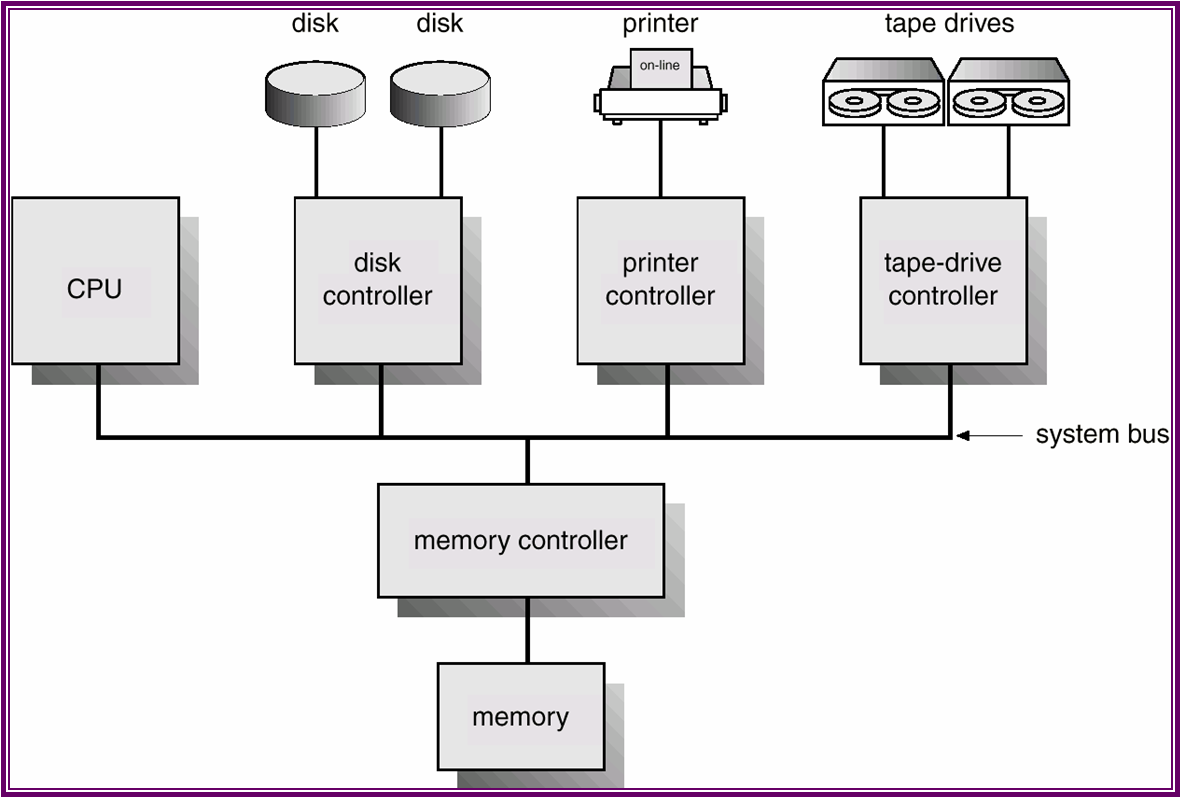
\includegraphics[scale=.35]{v6f2-1} \pause
    \end{center}
    \begin{itemize}
    \item{The CPU and device controllers can execute concurrently, competing for memory cycles.} \pause
    \item{To ensure orderly access to the memory, a memory controller is provided to synchronize access to the memory.}
    \end{itemize}
  \end{frame}

  \subsection{Bootstrap}

  %% PAGE
  \begin{frame}
    \frametitle{Bootstrap} \pause
    \begin{itemize}
    \item{When users just power on a computer, there is no already running operating system available.} \pause
      \begin{itemize}
      \item{We must load the operating system kernel from some persistent storages, such as disk and network server, to memory.} \pause
      \item{Then the control is transfered to the entry of the operating system with a very basic environment.} \pause
      \item{This procedure is named \textbf{bootstrap} (or simply \textbf{boot}) an operating system.} \pause
      \item{The program which boots the operating system is called \textbf{boot-loader}.} \pause
      \end{itemize}
    \item{Examples}
      \begin{itemize}
      \item{\textbf{NTLDR} - boot-loader for Windows NT/2000/XP (resides in C:$\backslash$).} \pause
      \item{\textbf{BOOTMGR} - boot-loader for Windows Vista/7/8/10 (resides in C:$\backslash$).} \pause
	      \begin{itemize}
          \item{Loads the C:$\backslash$Windows$\backslash$System32$\backslash$winload.exe who finally loads the kernel.}  \pause
	      \end{itemize}
      \item{\textbf{GRUB} - one of boot-loaders for the Unix/Linux.} \pause
        % \item{Question: Who loads the boot-loader?} \pause
      \end{itemize}
    %\item{Bear in mind that} \pause
    %  \begin{itemize}
    %  \item{\textbf{The boot-loader is NOT part of the operating system.}}
    %  \end{itemize}
    \end{itemize}
  \end{frame}

  %% PAGE
  \begin{frame}
    \frametitle{Questions}
    \begin{itemize}
    \item{Any questions?}
    \end{itemize}
    \begin{center}
      
\includegraphics[scale=.5]{question}
    \end{center}
  \end{frame}

  \subsection{Interrupt and Exception}

  %% PAGE
  \begin{frame}
    \frametitle{Interrupt} \pause
    \begin{itemize}
    \item{Modern computers and operating systems are \textbf{interrupt driven}.} \pause
      \begin{itemize}
        % \item{If there is nothing to do, the operating system will sit quietly, waiting for something to happen.} \pause
      \item{Peripheral devices use \textbf{interrupt} to signal the CPU that something has happened.} \pause
      \end{itemize}
    \item{When the CPU is interrupted, it must \textbf{serve the interrupt} by} \pause
      \begin{enumerate}
      \item{\emph{Hardware}: saves some of registers and branches to the \textbf{interrupt service routine (ISR)};} \pause
      \item{\emph{Assembly language procedure in ISR}: saves rest of registers if necessary and sets up a convenient environment;} \pause
      \item{\emph{C language procedure in ISR}: does serve the interrupt, typically reads and buffers input data from peripheral device;} \pause
      \item{\emph{C language procedure in ISR}: returns to the \emph{assembly language procedure in ISR};} \pause
      \item{\emph{Assembly language procedure in ISR}: restores saved registers and returns to the location being interrupted. }
      \end{enumerate}
    \end{itemize}
  \end{frame}

  %% PAGE
  \begin{frame}
    \frametitle{Interrupt Vector} \pause
    \begin{itemize}
    \item{Usually, a computer system has several peripheral devices.} \pause
    \item{When an interrupt occurs, CPU must know which device triggered it.} \pause
      \begin{itemize}
      \item{Computer system assigns each device an \emph{unique} interrupt request number (e.g., an 8-bit integer), or simply \textbf{IRQ}.} \pause
      \item{The addresses of all ISRs are collected into a table called \textbf{interrupt vector table}, or simply \textbf{IVT}.} \pause
      \item{When servicing an interrupt, CPU uses IRQ to index the interrupt vector to fetch the address of ISR and branches to it.}
      \end{itemize}
    \end{itemize}
  \end{frame}

  %% PAGE
  \begin{frame}
    \frametitle{Put them all together} \pause
    \begin{center}
      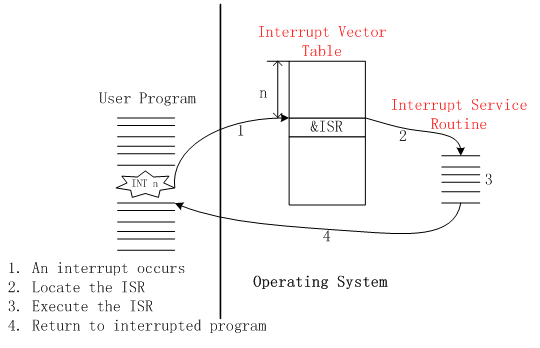
\includegraphics[scale=0.5]{isr}
    \end{center}
  \end{frame}

  %% PAGE
  \begin{frame}
    \frametitle{Exception} \pause
    \begin{itemize}
    \item{Interrupt} \pause
      \begin{itemize}
      \item{Triggered by peripheral devices;} \pause
      \item{Asynchronous.} \pause
      \end{itemize}
    \item{\textbf{Exception}} \pause
      \begin{itemize}
        % \item{Triggered by an error (such as division by zero and invalid memory access) \pause or by a specific request from a user program that an operating system service be performed.} \pause
      \item{Exceptions occur when the processor detects an error condition while executing an instruction, such as division by zero and invalid memory access.} \pause
      \item{Synchronous.} \pause
      \end{itemize}
    \item{Other than the above, handling of interrupts and exceptions is identical.} \pause
      \begin{itemize}
      \item{Exception is also known as \textbf{software-generated interrupt}
        or \textbf{synchronous interrupt}.}
      \end{itemize}
    \end{itemize}
  \end{frame}

  %% PAGE
  \begin{frame}
    \frametitle{Questions}
    \begin{itemize}
    \item{Any questions?}
    \end{itemize}
    \begin{center}
      
\includegraphics[scale=.5]{question}
    \end{center}
  \end{frame}

  \subsection{I/O structure}

\iffalse

  %% PAGE
  \begin{frame}
    \frametitle{I/O structure} \pause
    \begin{itemize}
    \item{When CPU is doing I/O with a peripheral device, two methods are available:} \pause
      \begin{itemize}
      \item{(a) synchronous \footnote{Also known as blocking or non-overlapping I/O.} \pause and (b) asynchronous \footnote{Also known as non-blocking or overlapping I/O.} I/O.} \pause
      \end{itemize}
    \end{itemize}
    \begin{center}
      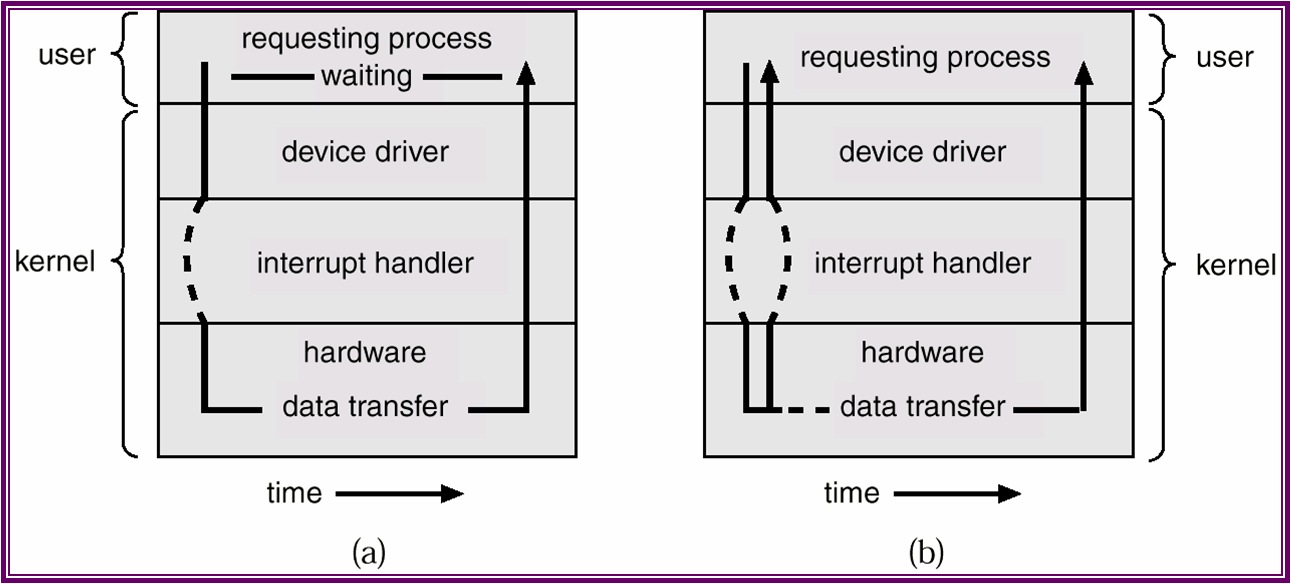
\includegraphics[scale=0.4]{v6f2-3}
    \end{center}
  \end{frame}

  %% PAGE
  \begin{frame}
    \frametitle{DMA (1/2)} \pause
    \begin{itemize}
    \item{Asynchronous I/O requires one interrupt per byte/word.} \pause
      \begin{itemize}
      \item{Even ISR is highly optimized, it does burn hundreds to thousands of CPU cycles.} \pause
      \item{This is unacceptable for high-speed devices, such as disk and network adapter.} \pause
      \end{itemize}
    \item{Here comes the DMA (Direct Memory Access).} \pause
      \begin{itemize}
      \item{After setting up addresses and counters for I/O device, the device controller transfers the entire block of data directly to or from its own buffer to memory, with no intervention by the CPU. } \pause
      \item{The DMA controller interrupts the CPU when the transfer has been completed.}
      \end{itemize}
    \end{itemize}
  \end{frame}

  %% PAGE
  \begin{frame}
    \frametitle{DMA(2/2)} \pause
    \begin{center}
      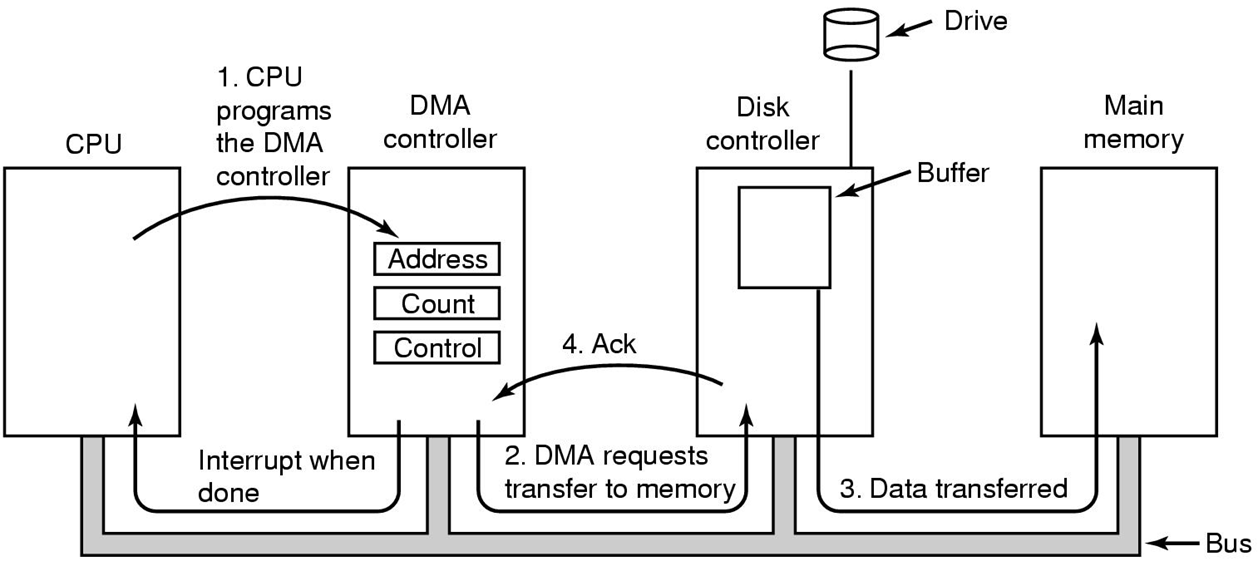
\includegraphics[scale=0.5]{mosv2f5-4}
    \end{center}
  \end{frame}

\fi

  %% PAGE
%  \begin{frame}
%    \frametitle{Example} \pause
%    \begin{center}
%      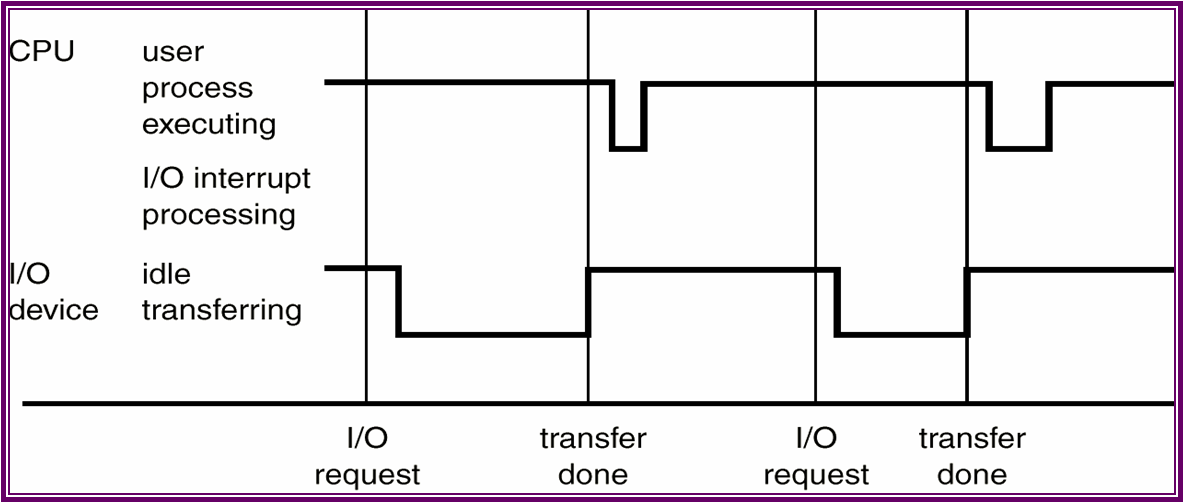
\includegraphics[scale=0.5]{v6f2-2}
%    \end{center}
%  \end{frame}

  %% PAGE
  \begin{frame}
    \frametitle{How CPU accesses peripheral devices?} \pause
    \begin{itemize}
    \item{CPU accesses devices through device controllers.} \pause
      \begin{itemize}
      \item{Device controllers include registers to hold commands and the data being transferred.} \pause
      \item{How CPU accesses these registers?} \pause
      \end{itemize}
    \item{Two methods:} \pause
      \begin{itemize}
      \item{I/O port} \pause
      \item{Memory-mapped I/O}
      \end{itemize}
    \end{itemize}
  \end{frame}

  %% PAGE
  \begin{frame}
    \frametitle{I/O port (1/2)} \pause
    \begin{itemize}
    \item{All registers within device controllers are collected.} \pause
      \begin{itemize}
      \item{An unique address (which is called \textbf{port}, an 8- or 16-bit integer) is assigned to each of them.} \pause
      \end{itemize}
    \item{Special I/O instructions are designed to allow data transfers between these registers and memory.} \pause
    \item{Example: IBM-PC} \pause
      \begin{itemize}
      \item{16-bit I/O ports are used to address the registers of device controllers.} \pause
      \item{Two special I/O instructions: \textbf{IN} and \textbf{OUT} are included in the INTEL x86 CPU.} \pause
        \begin{itemize}
        \item{IN \emph{reg}, \emph{port} - Read a byte/word from \emph{port} to CPU register \emph{reg}.} \pause
        \item{OUT \emph{port}, \emph{reg} - Write the content of CPU register \emph{reg} to \emph{port}.}
        \end{itemize}
      \end{itemize}
    \end{itemize}
  \end{frame}

  %% PAGE
  \begin{frame}
    \frametitle{I/O port (2/2)} \pause
    \begin{itemize}
    \item{Part of PC I/O port address map} \pause
    \end{itemize}
    \small
    \begin{center}
      \rowcolors[]{1}{blue!20}{blue!10}
      \begin{tabular}{ll} \hline
        \textbf{Range (hex)} & \textbf{Function}\\[0.5ex] \hline\hline
        000-01F & 1st DMA controller\\ \hline
        020-03F & 1st Programmable Interrupt Controller (PIC)\\ \hline
        040-05F & Programmable Interval Timer (System timer)\\ \hline
        060-06F & Keyboard\\ \hline
        220-233 & Sound card\\ \hline
        3D0-3DF & Color Graphics Adapter\\ \hline
      \end{tabular} \pause
    \end{center}
    \normalsize
    \begin{itemize}
    \item{Example: system timer} \pause
    \end{itemize}
    \begin{center}
      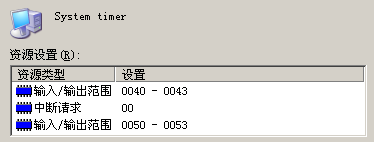
\includegraphics[scale=0.5]{ioportpit}
    \end{center}
  \end{frame}

  %% PAGE
  \begin{frame}
    \frametitle{Memory-mapped I/O (1/3)} \pause
    \begin{itemize}
    \item{In the method of I/O port,} \pause
      \begin{itemize}
      \item{we can view I/O ports as another separate address space, independent of memory address space.} \pause
      \end{itemize}
    \item{Registers within device controller is just a piece of storage.} \pause
      \begin{itemize}
      \item{Why not access these registers using the same method as memory?} \pause
      \item{In this case, a (unique) \textbf{memory address} is assigned to every register,\textbf{NOT a port address}.} \pause
      \end{itemize}
    \item{That's the memory-mapped I/O.} \pause
      \begin{itemize}
      \item{Memory-mapped I/O uses the same bus to address both memory and I/O devices} \pause
      \item{In order to accommodate the I/O devices, areas of CPU addressable space must be reserved for I/O rather than memory.}
      \end{itemize}
    \end{itemize}
  \end{frame}

  %% PAGE
  \begin{frame}
    \frametitle{Memory-mapped I/O (2/3)} \pause
    \begin{itemize}
    \item{Example: video controller of IBM-PC} \pause
      \begin{itemize}
      \item{Each location on the screen is mapped to a memory location.} \pause
      \end{itemize}
    \end{itemize}
    \begin{center}
      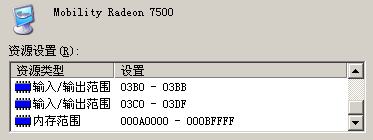
\includegraphics[scale=0.5]{ioportdisp}
    \end{center}
  \end{frame}

  %% PAGE
  \begin{frame}
    \frametitle{Memory-mapped I/O (3/3)} \pause
    \begin{itemize}
    \item{Advantages} \pause
      \begin{itemize}
      \item{Every instruction that can reference memory can also reference device controller registers.} \pause
        \begin{itemize}
        \item{The device drivers can be written entirely in C.} \pause
        \end{itemize}
      \item{No special protection mechanism is needed to keep user processes from performing I/O.} \pause
      \end{itemize}
    \item{Disadvantages} \pause
      \begin{itemize}
      \item{Most computers nowadays have some form of caching memory words. But, \pause caching a device controller register would be disastrous.} \pause
      \end{itemize}
    \item{Modern computer systems use both of them,} \pause
      \begin{itemize}
      \item{with memory-mapped I/O for data buffers and separate I/O ports for the command registers,} \pause
      \item{as in the previous example of \emph{Mobility Radeon 7500}.}
      \end{itemize}
    \end{itemize}
  \end{frame}

  %% PAGE
  \begin{frame}
    \frametitle{Questions}
    \begin{itemize}
    \item{Any questions?}
    \end{itemize}
    \begin{center}
      
\includegraphics[scale=.5]{question}
    \end{center}
  \end{frame}

\iffalse

  \subsection{Storage structure}

  %% PAGE
  \begin{frame}
    \frametitle{Storage structure} \pause
    \begin{center}
      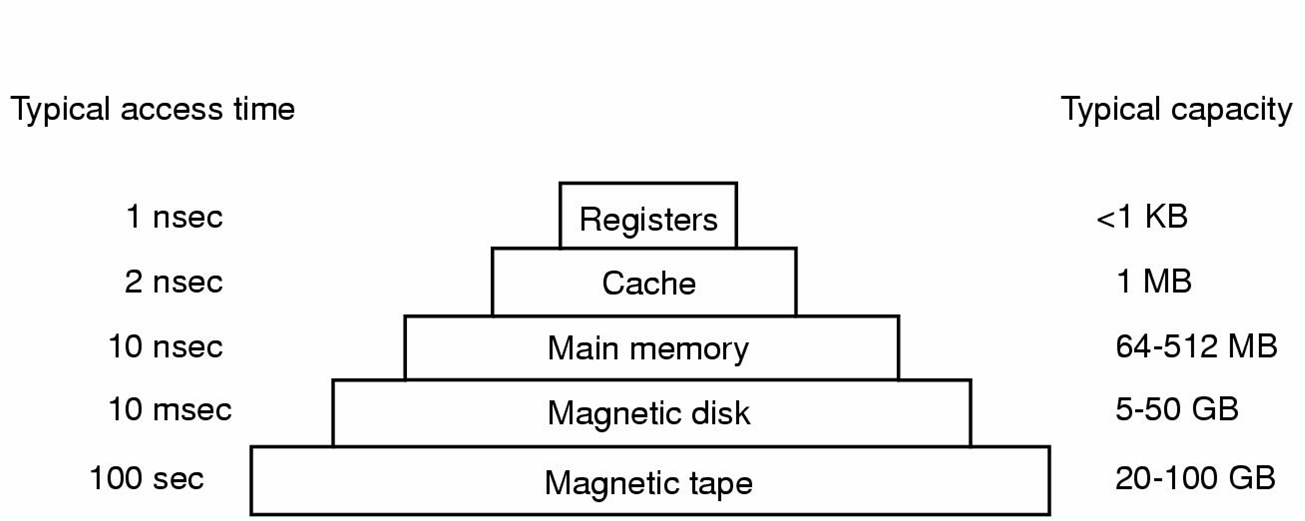
\includegraphics[scale=.5]{mosv2f1-7}\\
      Storage hierarchy \pause
    \end{center}
    \begin{itemize}
    \item{Computer program must be in main memory to be executed.} \pause
      \begin{itemize}
      \item{RAM is \textbf{volatile}, means it will lose its contents when the power to the device is removed.} \pause
      \end{itemize}
    \item{Data or program must be written to \textbf{nonvolatile} storage to be \textbf{persistent}.}
    \end{itemize}
  \end{frame}

  %% PAGE
  \begin{frame}
    \frametitle{Magnetic Disks} \pause
    \begin{center}
      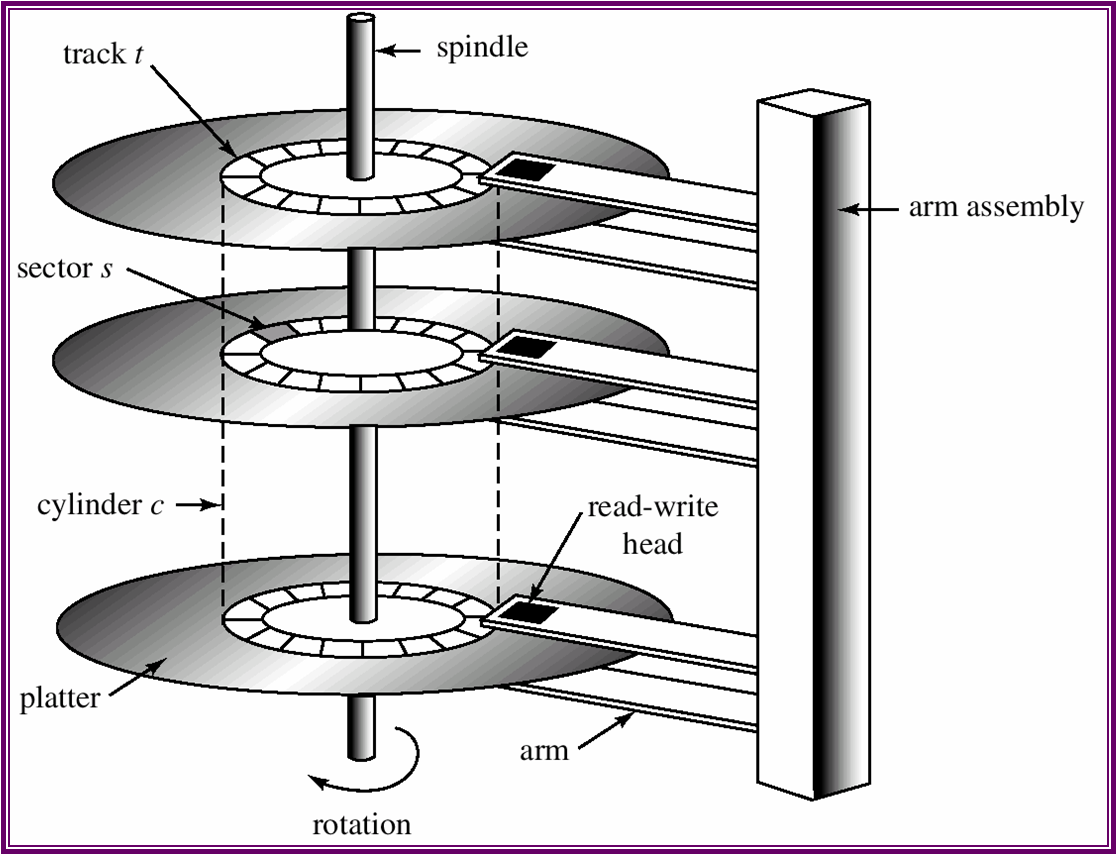
\includegraphics[scale=.3]{v6f2-5} \pause
    \end{center}
    \begin{itemize}
    \item{Every sector (also known as \textbf{disk block}) can be addressed by \textbf{(Cylinder, Head, Sector)}, or simply \textbf{CHS}.} \pause
      \begin{itemize}
      \item{sizeof(sector) = 512 bytes since 30 years ago \footnote{IDEMA recommended increasing the sector size from 512 bytes to 4096 in 2006.}.} \pause
      \end{itemize}
    \end{itemize}
  \end{frame}

  %% PAGE
  \begin{frame}
    \frametitle{Cache structure} \pause
    \begin{center}
      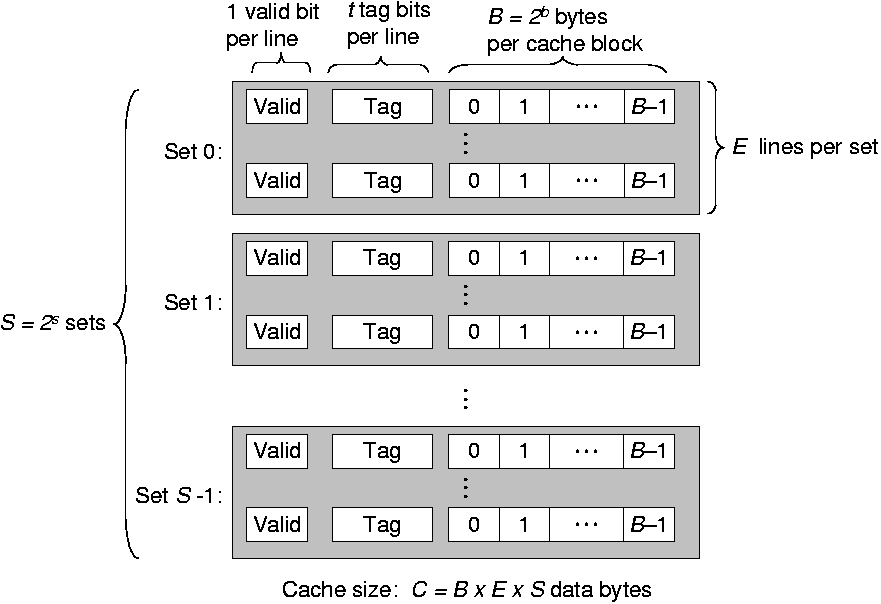
\includegraphics[scale=0.4]{csappv1f6-25}
    \end{center}
  \end{frame}

  %% PAGE
  \begin{frame}
    \frametitle{Accessing cache} \pause
    \begin{center}
      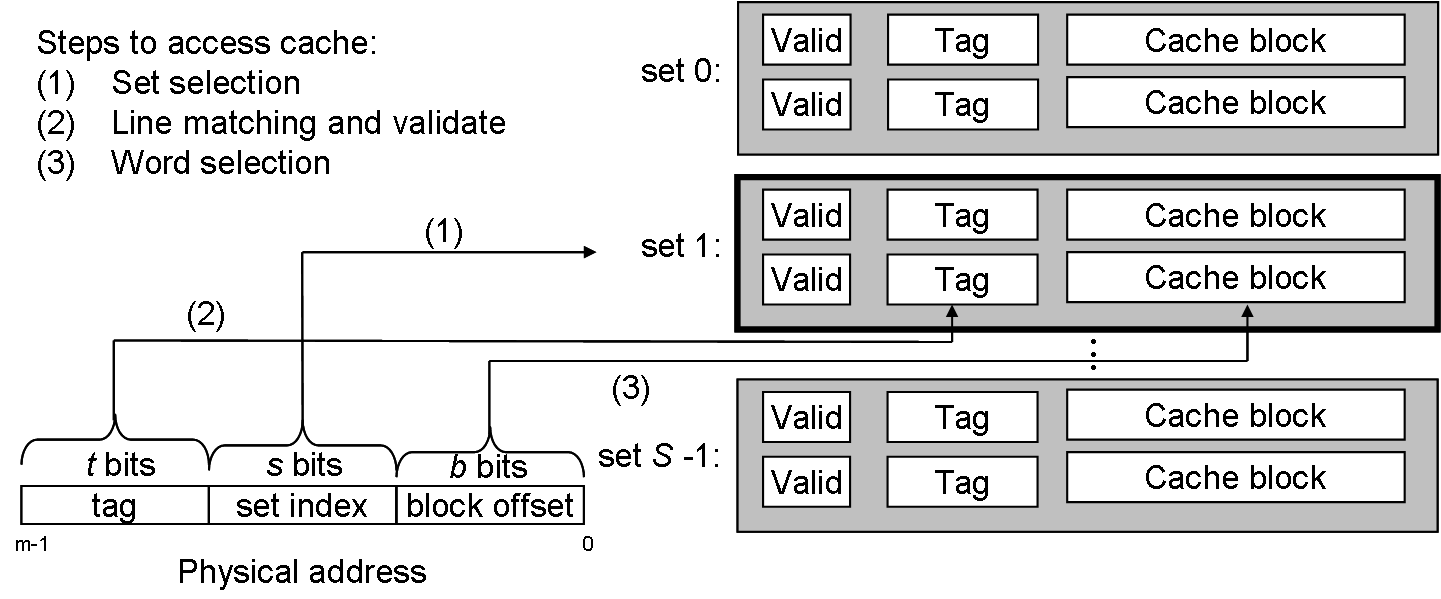
\includegraphics[scale=0.5]{csappv1f6-33}
    \end{center}
  \end{frame}

  %% PAGE
  \begin{frame}
    \frametitle{Cache types} \pause
    \begin{itemize}
    \item{Cache may be classified by different values of \textbf{E}, i.e., lines per set.} \pause
      \begin{itemize}
      \item{E = 1, \textbf{direct-mapped cache;}} \pause
      \item{$C/B>E>1$, \textbf{set associative cache};} \pause
        \begin{itemize}
        \item{\emph{E}-way associative cache} \pause
        \end{itemize}
      \item{$C/B=E$, \textbf{full associative cache}.} \pause
      \end{itemize}
      % \item{Example: Output of \emph{x86info}\footnote{A program used to dump IA-32 CPU detail information for Unix/Linux.} on a INTEL Pentium 4} \pause
      \begin{example}[Output of \emph{x86info} on a INTEL Pentium 4]
        \begin{quote}
          \small
          \textbf{Processor name string}: Intel(R) Pentium(R) 4 CPU 3.00GH\\
          \textbf{Cache info}\\
          Instruction trace cache: 12K uOps, 8-way associative.\\
          L1 Data cache: 16KB, sectored, 8-way associative. 64 byte line size.\\
          L2 unified cache: 2MB, sectored, 8-way associative. 64 byte line size.\\
          \textbf{TLB info}\\
          Instruction TLB: 4K, 2MB or 4MB pages, fully associative, 64 entries.\\
          Data TLB: 4KB or 4MB pages, fully associative, 64 entries.\\
          \normalsize
        \end{quote}
      \end{example}
    \end{itemize}
  \end{frame}

\fi

  %% PAGE
  \begin{frame}
    \frametitle{Questions}
    \begin{itemize}
    \item{Any questions?}
    \end{itemize}
    \begin{center}
      
\includegraphics[scale=.5]{question}
    \end{center}
  \end{frame}

  \subsection{Hardware protection}

  %% PAGE
  \begin{frame}
    \frametitle{Hardware protection} \pause
    \begin{itemize}
    \item{To ensure proper operation, we must protect the operating system and all other program and their data from any malfunctioning program.} \pause
    \item{Hardware protection can be broken down different ways} \pause
      \begin{itemize}
      \item{\textbf{Dual-mode operation} \pause - Prevent user programs taking over part of the OS and using this to overwrite other programs or even modify the OS itself.} \pause
      \item{\textbf{Privileged instructions} \pause - Prevent user programs disrupting the normal operation of the system by issuing illegal I/O instructions.} \pause
      \item{\textbf{Memory protection} \pause - Prevent a user program directly accessing the memory of another user program  or even operating system.} \pause
      \item{\textbf{CPU protection} \pause - Prevent a user program from getting stuck in an infinite loop and never returning control to the operating system.}
      \end{itemize}
    \end{itemize}
  \end{frame}

  %% PAGE
  \begin{frame}
    \frametitle{Dual-mode operation} \pause
    \begin{itemize}
    \item{We need at least two separate modes of operation:} \pause
      \begin{itemize}
      \item{\textbf{User mode} \pause - Execution on behalf of user programs;} \pause
      \item{\textbf{Monitor mode} \pause - Execution on behalf of operating system.} \pause
        \begin{itemize}
        \item{Also known as \textbf{supervisor, system, privileged or kernel mode}.} \pause
        \end{itemize}
      \end{itemize}
    \item{\textbf{Mode bit} is added to computer hardware to indicate the current mode:  monitor (0) or user (1).} \pause
      \begin{itemize}
      \item{It's set to \emph{monitor} at system boot time. \pause The operating system is then loaded, and starts user programs in user mode.} \pause
      \end{itemize}
    \item{When an interrupt or exception occurs hardware switches to monitor mode.} \pause
      \begin{itemize}
      \item{Whenever the operating system gains control of the computer, it's in monitor mode.} \pause
      \item{And the system always switches to user mode before passing control to a user program.}
      \end{itemize}
    \end{itemize}
  \end{frame}

  %% PAGE
  \begin{frame}
    \frametitle{Example} \pause
    \begin{itemize}
    \item{INTEL IA-32 supports 4 modes to operate, named \textbf{protection rings}.} \pause
    \end{itemize}
    \begin{center}
      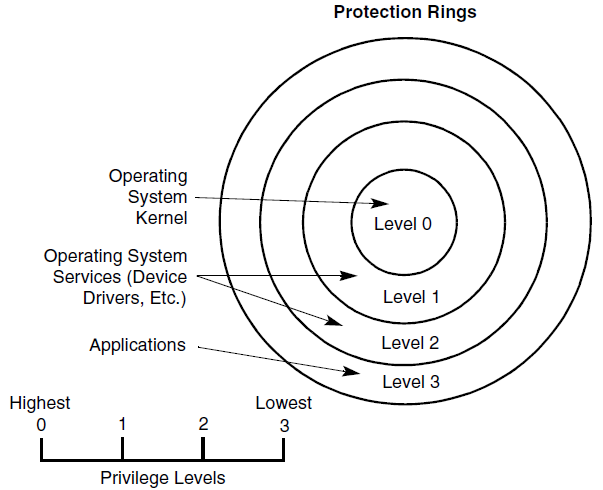
\includegraphics[scale=0.3]{x86rings} \pause
    \end{center}
    \begin{itemize}
    \item{But, most operating systems running on IA-32 only use 2 of 4.} \pause
      \begin{itemize}
      \item{Ring 0 as monitor mode; \pause ring 3 as user mode.}
      \end{itemize}
    \end{itemize}
  \end{frame}

   %% PAGE
  \begin{frame}
    \frametitle{Example (cont'd)} \pause
    \begin{itemize}
    \item{\textbf{Mode bit} of INTEL IA-32} \pause
    \end{itemize}
    \begin{center}
      \setlength{\unitlength}{.5cm}
      \begin{picture}(20, 14)
        \color{red}
        \put(0, 0){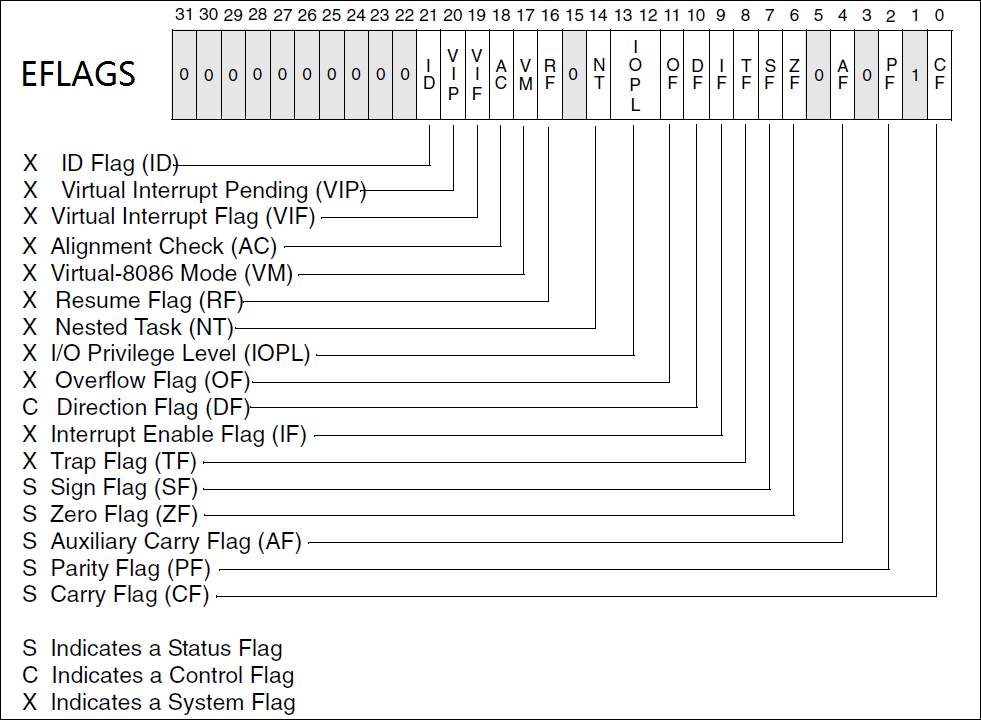
\includegraphics[scale=.35]{x86eflags}} \pause
        \put(0, 6.6){\framebox(6, 0.45){}}
      \end{picture}
    \end{center}
  \end{frame}

  %% PAGE
  \begin{frame}
    \frametitle{I/O protection} \pause
    \begin{itemize}
    \item{All I/O instructions are privileged instructions.} \pause
      \begin{itemize}
      \item{The hardware allows privileged instructions to be executed only in monitor mode.} \pause
      \item{If these instructions are to be executed in user mode, the
        hardware does not execute the instruction, but rather treats it as
      illegal and generates an exception.} \pause
      \item{For example, \textbf{IN} and \textbf{OUT} are 2 privileged instructions in INTEL IA-32.} \pause
      \end{itemize}
    \item{Must ensure that a user program could never gain control of the computer in monitor mode. }
    \end{itemize}
  \end{frame}

  %% PAGE
  \begin{frame}
    \frametitle{Memory protection} \pause
    \begin{itemize}
    \item{In order to have memory protection, add two registers that determine the range of legal addresses a program may access:} \pause
      \begin{itemize}
      \item{\textbf{Base register} \pause - holds the smallest legal physical memory address;} \pause
      \item{\textbf{Limit register} \pause - contains the size of the range.} \pause
      \end{itemize}
      % \item{Memory outside the defined range is protected.} \pause
    \end{itemize}
    \begin{center}
      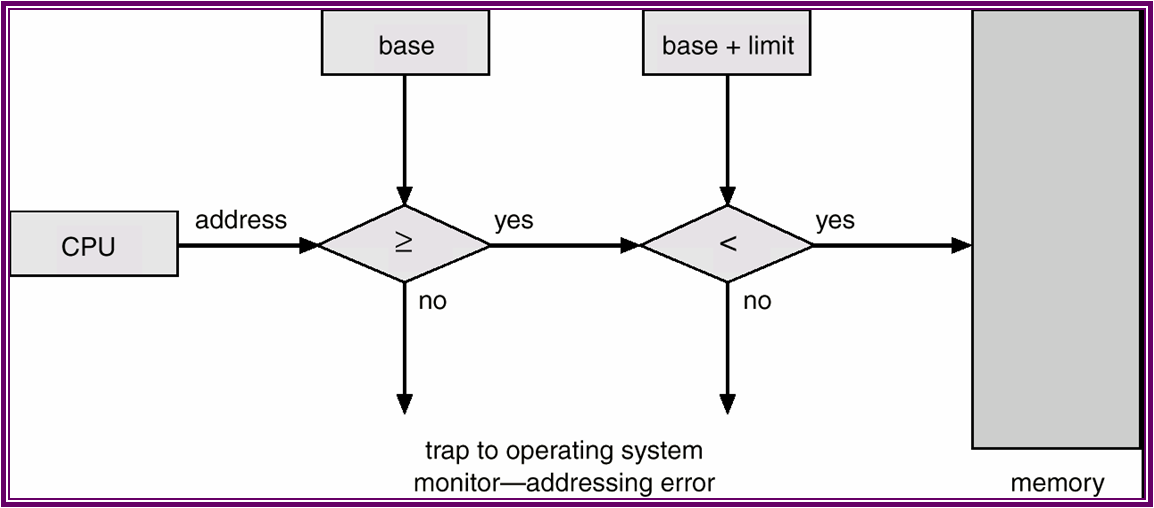
\includegraphics[scale=0.4]{v6f2-10} \pause
    \end{center}
    \begin{itemize}
    \item{We will return to this topic when entering \emph{memory management}.}
    \end{itemize}
  \end{frame}

  %% PAGE
  \begin{frame}
    \frametitle{Example} \pause
    \begin{center}
      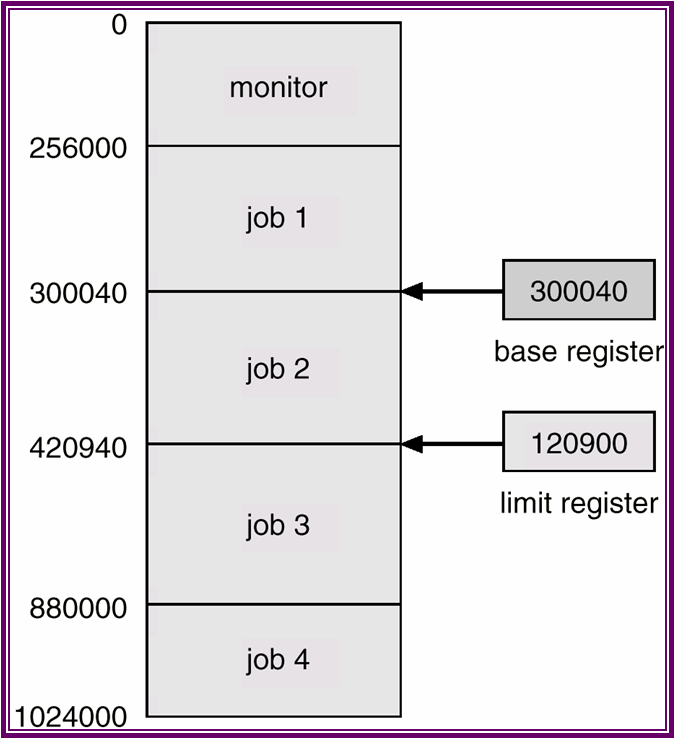
\includegraphics[scale=0.5]{v6f2-9}
    \end{center}
  \end{frame}

  %% PAGE
  \begin{frame}
    \frametitle{CPU protection} \pause
    \begin{itemize}
    \item{The operating system can enforce policies only if it gets a chance to run.} \pause
      \begin{itemize}
      \item{If a malfunctioning program entered an infinite loop and never returns control to the operating system, then CPU was out of the control from the operating system.} \pause
      \end{itemize}
    \item{\textbf{Timer} \pause - interrupts CPU after a specified period to ensure operating system maintains control.} \pause
      \begin{itemize}
      \item{Remember that when interrupt occurs, the operating system will get the control via ISR.} \pause
      \end{itemize}
%    \item{The timer can also be used to implement time sharing.}
    \end{itemize}
  \end{frame}

  %% PAGE
  \begin{frame}
    \frametitle{Timer} \pause
    \begin{center}
      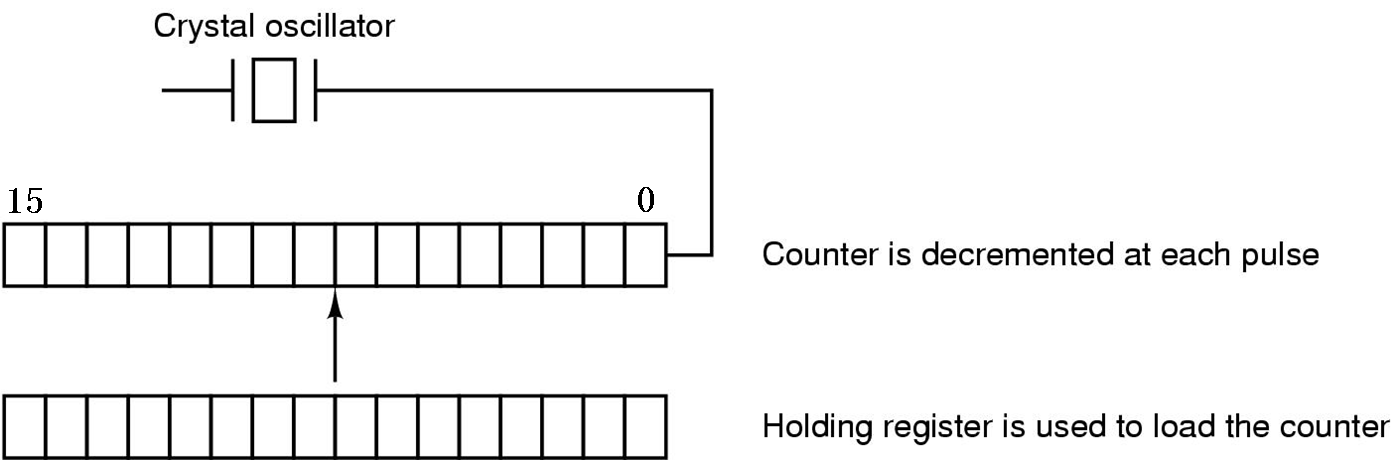
\includegraphics[scale=.2]{mosv2f5-31} \pause
    \end{center}
    \begin{itemize}
    \item{The \emph{counter register} is decremented by 1 at each pulse.} \pause
      \begin{itemize}
      \item{When the \emph{counter register} reaches zero, the timer will interrupt CPU.} \pause
      \item{Then the \emph{counter register} will be reloaded with the value of \emph{holding register} and decrementing repeats.} \pause
      \end{itemize}
    \item{Example: Timer in IBM-PC} \pause
      \begin{itemize}
      \item{An INTEL i8253 programmable interval timer with 16-bit counter and holding registers and pulses reach at 1193182Hz.}
      \end{itemize}
    \end{itemize}
    % \begin{center}
    %   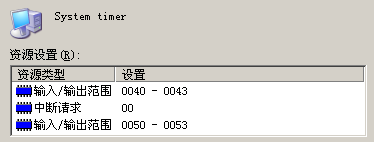
\includegraphics[scale=0.5]{ioportpit}
    % \end{center}

  \end{frame}

  %% PAGE
  \begin{frame}
    \frametitle{Questions}
    \begin{itemize}
    \item{Any questions?}
    \end{itemize}
    \begin{center}
      
\includegraphics[scale=.5]{question}
    \end{center}
  \end{frame}

  \subsection{System call}

  %% PAGE
  \begin{frame}
    \frametitle{System call} \pause
    \begin{itemize}
    \item{The operating system does nothing useful itself.} \pause
      \begin{itemize}
      \item{But it provides some useful services to the user programs, such as reading a file from disk and sending data to remote host via network adapter.} \pause
      \item{How does operating system provide these services?} \pause
      \end{itemize}
    \item{It's the \textbf{system call} \pause - the (well-defined) \textbf{interface} between the operating system and the user programs.} \pause
      \begin{itemize}
      \item{User programs can \textbf{ONLY} request services provided by the operating system via system call.} \pause
      \item{The system calls in the interface vary from operating system to operating system.} \pause
      \item{Also known as \textbf{supervisor call}.}
      \end{itemize}
      % \item{We will explain system call in detail by an example.}
    \end{itemize}
  \end{frame}

  %% PAGE
  \begin{frame}
    \frametitle{Example} \pause
    \begin{itemize}
    \item{Most operating systems provide the service that can read some bytes from a file: \emph{read}} \pause
      \begin{itemize}
      \item{\emph{count = read(fd, buffer, nbytes);}} \pause
      \item{This system call reads \emph{nbytes} data from file \emph{fd} to the specified \emph{buffer} and returns the number of bytes actually read in \emph{count}.}
      \end{itemize}
      % \item{You may treat it as a \textbf{library call} as usual.} \pause
      %   \begin{itemize}
      %   \item{But there is a sharp difference: \textbf{the system calls will
        %   trap into the operating system, while library calls do NOT}. } \pause
      %   \end{itemize}
    \end{itemize}
  \end{frame}

  %% PAGE
  \begin{frame}
    \frametitle{Procedure (1/2)} \pause
    \small
    \begin{minipage}[c]{0.45\textwidth}
      \begin{enumerate}
      \item[1-3]{Prepare parameters;} \pause
      \item[4]{Call the wrapper (written in assembly language) of system call;} \pause
      \item[5]{Store the \textbf{system call number} of \emph{read} into a register;} \pause
      \item[6]{Trap into the operating system;} \pause
      \item[7]{Get \textbf{system call service routine} for \emph{read} by indexing a \textbf{system call table} using system call number;} \pause
      \item[8-11]{System call service routine runs and returns to user programs on completion.} \pause
      \end{enumerate}
    \end{minipage}%
    \begin{minipage}[c]{0.55\textwidth}
      \begin{center}
        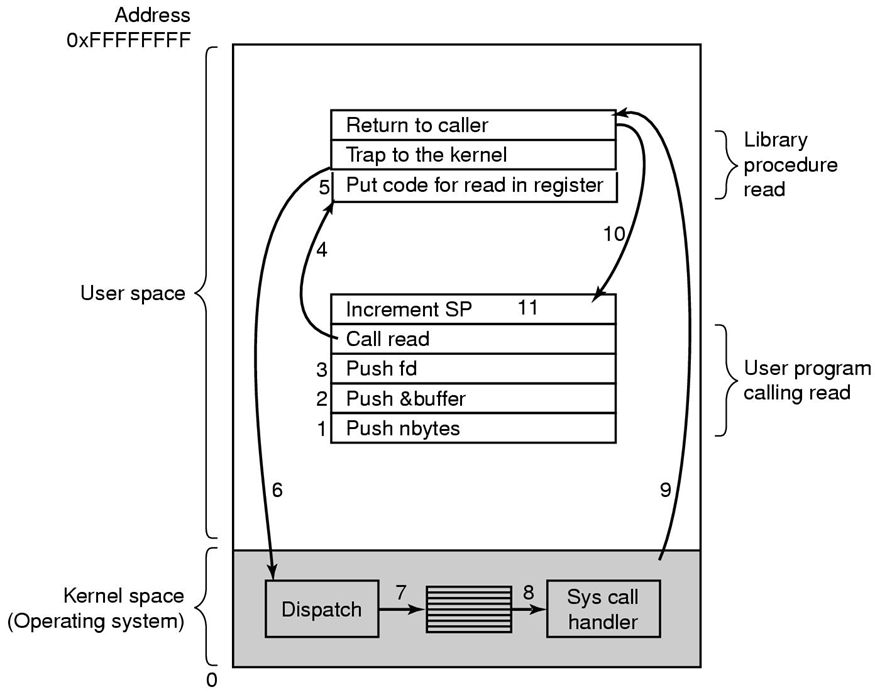
\includegraphics[scale=0.45]{mosv2f1-17}
      \end{center}
    \end{minipage}
    \normalsize
  \end{frame}

  %% PAGE
  \begin{frame}
    \frametitle{Procedure (2/2)} \pause
    \begin{center}
      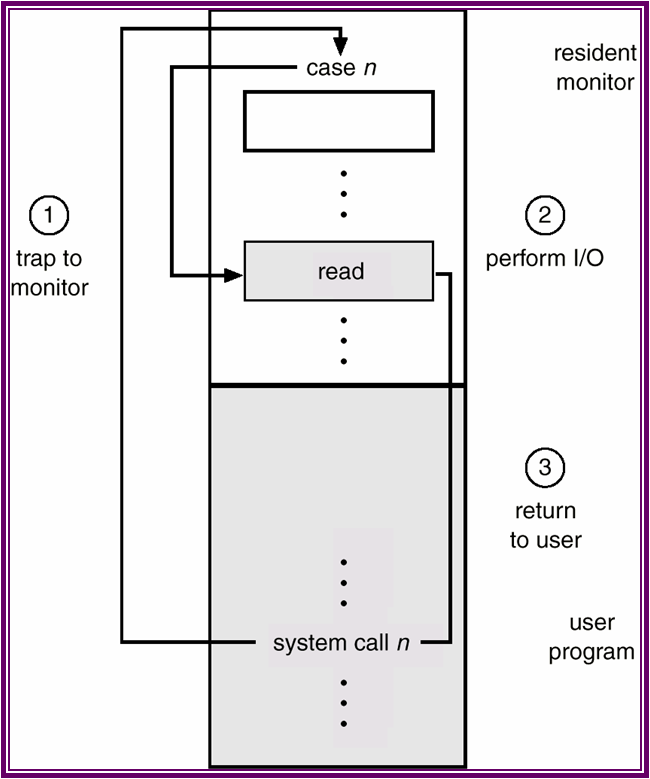
\includegraphics[scale=.4]{v6f2-8} \pause
    \end{center}
    \begin{itemize}
    \item{Resident monitor (or simply monitor) here means the operating system and} \pause
    \item{\emph{n} is the system call number.}
    \end{itemize}
  \end{frame}

  %% PAGE
  \begin{frame}
    \frametitle{Trap into the operating system (1/2)} \pause
    \begin{itemize}
    \item{The user programs cannot trap into the operating system directly.} \pause
    \item{How to trap into the operating system?} \pause
      \begin{itemize}
      \item{Method 1: \textbf{Exception (software-generated interrupt)}.} \pause
      \item{Method 2: Special instruction.}
      \end{itemize}
    \end{itemize}
  \end{frame}

  %% PAGE
  \begin{frame}
    \frametitle{Trap into the operating system (2/2)} \pause
    \begin{itemize}
    \item{Exception} \pause
      \begin{itemize}
      \item{INTEL IA-32 provides an instruction to trigger a exception, \emph{INT}.} \pause
        \begin{itemize}
        \item{For example, FreeBSD/Linux uses \emph{INT 0x80} to trap into the operating system and Windows NT/XP uses \emph{INT 0x2e}.} \pause
        \end{itemize}
      \end{itemize}
    \item{Special instruction} \pause
      \begin{itemize}
      \item{In addition, INTEL IA-32 provides two special instructions to trap into the operating system: \emph{SYSENTER and SYSEXIT} because of the extra overhead of \emph{INT} instruction.} \pause
        \begin{itemize}
        \item{Only supported on processors after Pentium II, i.e., Family 6, Model 3, Stepping 3.} \pause
        \end{itemize}
      \item{ARM processors use \emph{swi} \footnote{Short for SoftWare
        Interrupt.} to trap into the operating system.}
      \end{itemize}
    \end{itemize}
  \end{frame}

  %% PAGE
  \begin{frame}
    \frametitle{System call v.s. library function} \pause
    \begin{itemize}
    \item{System call will trap into the OS kernel; while library function does not.} \pause
      \begin{itemize}
      \item{So, system call is MUCH more slow than library function.} \pause
      \end{itemize}
    \item{Library function is the same as the user-defined function. We can replace an existing library function with our own versions, but we can't replace a system call.} \pause
    \item{A system call in one operating system may become a library function in another operating system and vice versa.} \pause
    \end{itemize}
    \begin{center}
      \includegraphics[scale=.4]{syscallvslibcall}
    \end{center}
  \end{frame}

  %% PAGE
  \begin{frame}
    \frametitle{Questions}
    \begin{itemize}
    \item{Any questions?}
    \end{itemize}
    \begin{center}
      
\includegraphics[scale=.5]{question}
    \end{center}
  \end{frame}

  \subsection{Function calling convention in C}

  %% PAGE
  \begin{frame}[fragile]
    \frametitle{Function calling convention in C} \pause
    \begin{minipage}[c]{0.4\textwidth}
\begin{lstlisting}
int foo(int a, int b)
{
     char buf[4];
     return a+b;
}
int main()
{
     int i;
     i = foo(12, 34);
     return i;
}
\end{lstlisting}
      \pause
    \end{minipage}%
    \begin{minipage}[c]{0.6\textwidth}
      \setlength{\unitlength}{0.5cm}
      \begin{picture}(10, 10)
        \put(4, 0){\line(0, 1){10}}
        \put(8, 0){\line(0, 1){10}}
        \put(8.5, 0){Low addr.}
        \put(8.5, 9.5){High addr.}
        \put(5, 2){\vector(-1, 0){1}}
        \put(5.5, 1.8){4B}
        \put(7, 2){\vector(1, 0){1}}
        \put(5, 0.1){Stack}

        \pause

        \put(4, 8){\framebox(4, 1){34}} \pause
        \put(4, 7){\framebox(4, 1){12}} \pause
        \put(4, 6){\framebox(4, 1){return addr.}} \pause
        \put(4, 5){\framebox(4, 1){old fp}}\pause
        \put(2.3, 5.4){fp} \pause
        \put(4, 4){\framebox(1, 1){[3]}}
        \put(5, 4){\framebox(1, 1){[2]}}
        \put(6, 4){\framebox(1, 1){[1]}}
        \put(7, 4){\framebox(1, 1){[0]}} \pause
        \put(8, 4.4){ buf} \pause
        \put(4, 3){\framebox(4, 1){......}} \pause
        \put(2.6, 6.4){+4 } \pause
        \put(2.6, 7.4){+8 } \pause
        \put(2.6, 8.4){+c } \pause
        \put(2.8, 4.4){-4 } \pause

        \color{red}\put(3.9, 2.9){\framebox(4.2, 6.2){}}\color{black} \pause
      \end{picture}
      \begin{itemize}
      \item{The area enclosed by red rectangle is called \textbf{stack frame}, or simply \textbf{frame}.} \pause
        \begin{itemize}
        \item{Stack frames are chained into a singly-linked list via \textbf{fp} (short for \textbf{frame pointer}).}
        \end{itemize}
      \end{itemize}
    \end{minipage}
\end{frame}

  %% PAGE
  \begin{frame}
    \frametitle{Stack frame} \pause
    \begin{itemize}
    \item{The stack frame (also known as \textbf{activation record}) is used to record the information of function calling.} \pause
      \begin{itemize}
      \item{Parameters} \pause
      \item{Return address} \pause
      \item{Local variables allocation and} \pause
      \item{a ``prev'' pointer to previous stack frame.} \pause
      \end{itemize}
    \item{It's stored in the \textbf{stack} of the running program.}
    \end{itemize}
  \end{frame}

  %% PAGE
  \begin{frame}
    \frametitle{Questions}
    \begin{itemize}
    \item{Any questions?}
    \end{itemize}
    \begin{center}
      
\includegraphics[scale=.5]{question}
    \end{center}
  \end{frame}

  %% PAGE
\end{CJK*}
\end{document}
